%
% Capítulo 5
%
\chapter{Conclusões} \label{cap5}

Neste capítulo apresentam-se as conclusões relativas ao desempenho e trabalho realizado pelo grupo. São efetuadas comparações face ao planeamento inicial previsto e ao que realmente sucedeu, como forma de analisar e apreciar o trabalho realizado.

\section{Planeamento}\label{sec51}

Na Figura \ref{planning} está representado o planeamento ao longo do projeto, igualmente, estão as percentagens de trabalho realizado em cada um dos principais pontos. As datas críticas do projeto estão também presentes na Figura \ref{planning}, de modo a que se possa observar da melhor maneira as tarefas e prazos a cumprir.

Tentou-se, ao máximo, que o maior número de tarefas pudesse ser executado em paralelo, para assim aumentar a eficiência e melhor gerir os recursos disponíveis. Essencialmente as tarefas foram dividas de acordo com a camada/bloco onde se encontravam, sendo requisito, o seu desenvolvimento, teste e documentação.


Note-se que a partir da semana catorze até à semana da entrega final, as tarefas a realizar dependerão vivamente da qualidade da entrega da versão beta. Servirá também para melhoramentos, visto que a melhoria se trata de um processo contínuo. Eventualmente os requisitos funcionais não entregues na versão beta, serão executados também no decorrer desse período.
 

\begin{figure}
	\hspace{-1.75cm}
	\resizebox{19cm}{23cm}{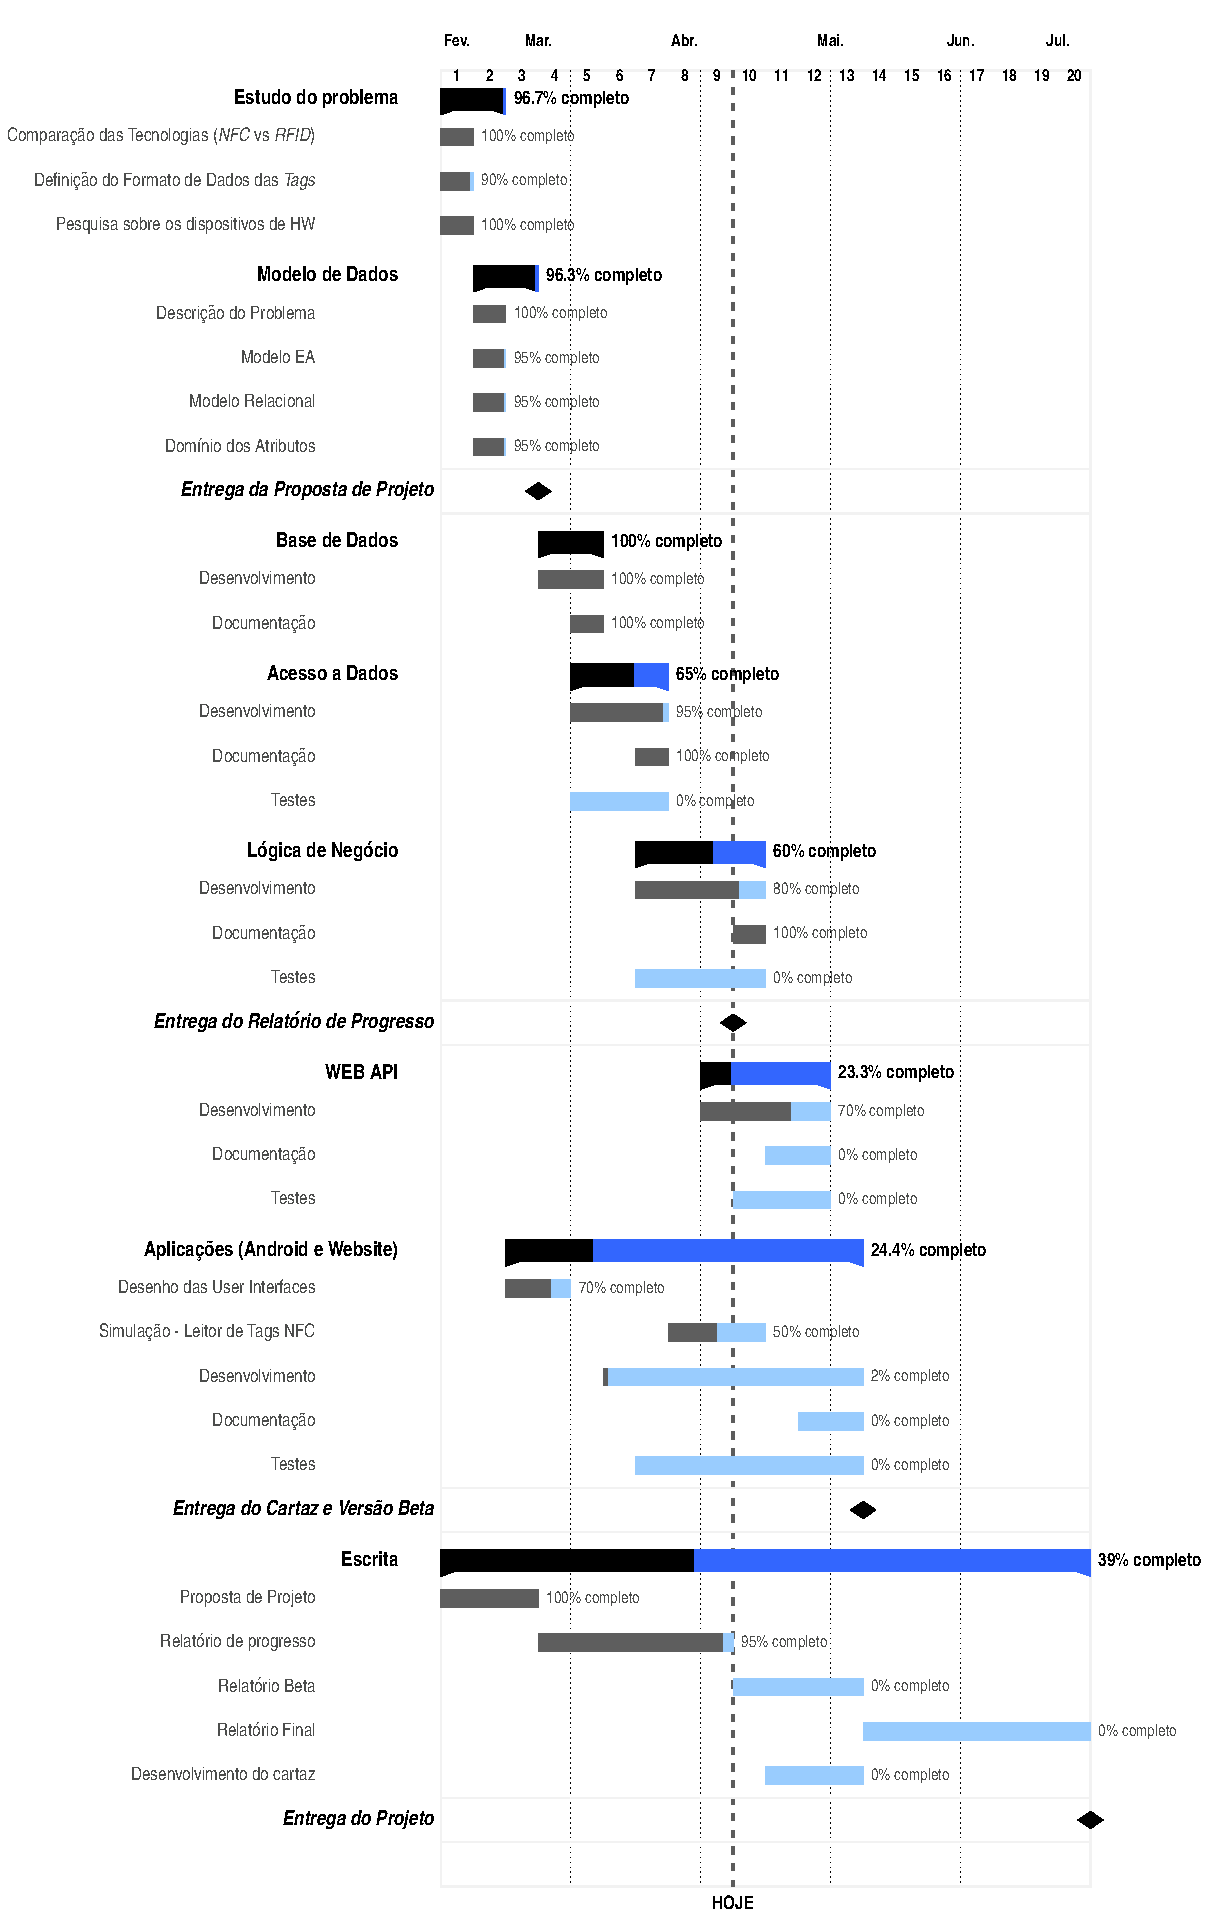
\includegraphics{./files/Planeamento.pdf}}
	\caption{Planeamento}
	\label{planning}
\end{figure}

\section{Sumário}\label{sec52}

Nas semanas iniciais foi realizada pesquisa de forma a melhor entender conceitos, dificuldades e potenciais resoluções e/ou abordagens. 

De seguida definiu-se o problema e como seria solucionado, tendo também sido apresentada a proposta de projeto publicamente.

A partir das seguintes datas, começou-se a efetiva implementação das várias camadas. Até à data foram desenvolvidas as camadas: \acrlong{bd}, Acesso a Dados, Lógica de Negócio e iniciada a \gls{api-web}. De forma geral os requisitos foram cumpridos. Foi notado um ligeiro atraso de, aproximadamente, uma semana em relação ao planeamento esperado.

\section{Trabalho Futuro}\label{sec53}

Existe ainda trabalho crucial por realizar, nomeadamente a \gls{api-web} e as aplicações móvel e \textit{web}. Seria deveras importante recuperar o atraso que se fez sentir até agora, pelo que será necessário um esforço adicional pelo grupo de trabalho.